\documentclass{article}
\usepackage{physics}
\usepackage{tikz}        
\usepackage{amsmath, amsfonts}
\usepackage{empheq}
\usepackage{mathtools}

\newcommand*\widefbox[1]{\fbox{\hspace{2em}#1\hspace{2em}}} % boxing equations
\newcommand{\egreg}{\vphantom{-}} % vertical spacing for subscripts

\title{Physics 223b: Advanced Condensed Matter Physics}
\date{Spring 2022}
\author{Mathias Driesse}
\begin{document}
    

\begin{titlepage}
    \maketitle
    
\end{titlepage}

\section{Course Overview: Superfluids and Super conductors}

Superfluids and superconductors are considered by many to be the greatest all-time condensed matter discovery, which resulted in Nobel Prizes in the yeras 1913, 1962, 1972, 1972, 1973, 1978, 1987, 1996 and 2003!





\tikzset{every picture/.style={line width=0.75pt}} %set default line width to 0.75pt        

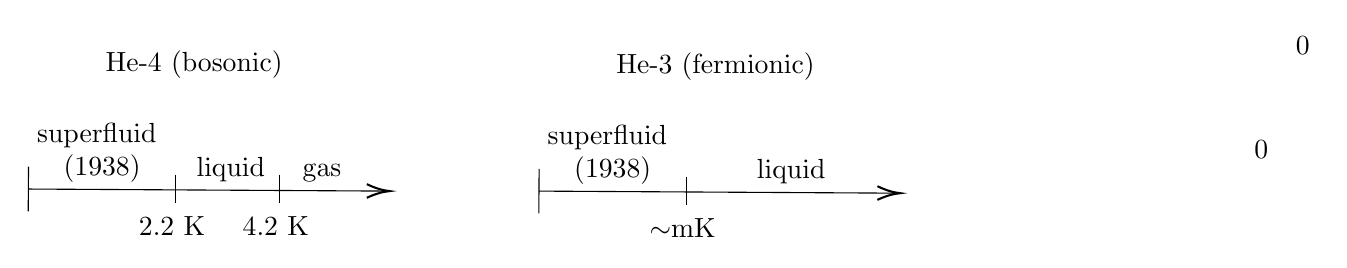
\begin{tikzpicture}[x=0.75pt,y=0.75pt,yscale=-1,xscale=1]
%uncomment if require: \path (0,790); %set diagram left start at 0, and has height of 790

%Straight Lines [id:da05397847095677921] 
\draw    (107,90) -- (279,90.99) ;
\draw [shift={(281,91)}, rotate = 180.33] [color={rgb, 255:red, 0; green, 0; blue, 0 }  ][line width=0.75]    (10.93,-3.29) .. controls (6.95,-1.4) and (3.31,-0.3) .. (0,0) .. controls (3.31,0.3) and (6.95,1.4) .. (10.93,3.29)   ;
%Straight Lines [id:da7149073367988203] 
\draw    (107.07,79.25) -- (106.93,100.75) ;
%Straight Lines [id:da4846479461755506] 
\draw    (178,83) -- (178,96.6) ;
%Straight Lines [id:da37923163818797456] 
\draw    (228,83) -- (228,96.6) ;
%Straight Lines [id:da31574591578223865] 
\draw    (353,91) -- (525,91.99) ;
\draw [shift={(527,92)}, rotate = 180.33] [color={rgb, 255:red, 0; green, 0; blue, 0 }  ][line width=0.75]    (10.93,-3.29) .. controls (6.95,-1.4) and (3.31,-0.3) .. (0,0) .. controls (3.31,0.3) and (6.95,1.4) .. (10.93,3.29)   ;
%Straight Lines [id:da36960515655446846] 
\draw    (353.07,80.25) -- (352.93,101.75) ;
%Straight Lines [id:da35915116487668874] 
\draw    (424,84) -- (424,97.6) ;

% Text Node
\draw (721,21) node    {$0$};
% Text Node
\draw (701,71) node    {$0$};
% Text Node
\draw (143,22) node [anchor=north west][inner sep=0.75pt]   [align=left] {He-4 (bosonic)};
% Text Node
\draw (204.52,88) node [anchor=south] [inner sep=0.75pt]   [align=left] {liquid};
% Text Node
\draw (142.52,88) node [anchor=south] [inner sep=0.75pt]   [align=left] {\begin{minipage}[lt]{46.95pt}\setlength\topsep{0pt}
superfluid
\begin{center}
(1938)
\end{center}

\end{minipage}};
% Text Node
\draw (248.49,88) node [anchor=south] [inner sep=0.75pt]   [align=left] {gas};
% Text Node
\draw (159,102) node [anchor=north west][inner sep=0.75pt]   [align=left] {2.2 K};
% Text Node
\draw (209,102) node [anchor=north west][inner sep=0.75pt]   [align=left] {4.2 K};
% Text Node
\draw (389,23) node [anchor=north west][inner sep=0.75pt]   [align=left] {He-3 (fermionic)};
% Text Node
\draw (474.52,89) node [anchor=south] [inner sep=0.75pt]   [align=left] {liquid};
% Text Node
\draw (388.52,89) node [anchor=south] [inner sep=0.75pt]   [align=left] {\begin{minipage}[lt]{46.95pt}\setlength\topsep{0pt}
superfluid
\begin{center}
(1938)
\end{center}

\end{minipage}};
% Text Node
\draw (405,103) node [anchor=north west][inner sep=0.75pt]   [align=left] {$\sim$mK};

\end{tikzpicture}

Besides in He-4 and He-3, superfluids have also been realized in ultracold bosonic/fermionic atoms (Rb, Li, Na, ...).

% more diagram



Superfluids and superconductors are deeply related macroscopic quantum phenomena with vast technological promise:
\begin{itemize}
    \item Stable high $\vec{B}$-field generation (MRIs)
    \item Magnetic levitation
    \item Magnetometry (SQUIDs)
    \item Power transmission
    \item Dark matter detection
    \item Quantum computation (superconducting qubits)          
\end{itemize}

There are many varieties, ranging from "conventional" to exotic (e.g., topological superconductors). Understanding them is key to many branches of modern quantum science!

\underline{This quarter:} Superfluidity $\rightarrow$ superconductivity, emphasizing broader phenomenology, microscopic underpinnings, and some applications/frontier topics. Let us proceed with...

\section{The Bose-Hubbard Model}\label{The Bose-Hubbard Model} 

Take bosons on a 2D\footnote{The dimensionality is important...} square lattice\footnote{...But the precise lattice is not so important.}.

% insert diagram here

We use the canonical boson operators $b_{\vec{r}}^{\dagger}$, $b_{\vec{r}}^{\egreg}$, with the commutation relations

\begin{empheq}[box=\widefbox]{align*}
    [b_{\vec{r}}^{\egreg}, b_{\vec{r}'}^{\dagger}] = \delta_{\vec{r}, \vec{r}'}, \quad [b_{\vec{r}}^{\egreg}, b_{\vec{r}'}^{\egreg}] = [b_{\vec{r}'}^{\dagger}, b_{\vec{r}'}^{\dagger}] = 0 \\
    n_{\vec{r}} = b_{\vec{r}}^{\dagger}b_{\vec{r}}^{\egreg} = \textrm{boson occupation number} \\
    b_{\vec{r}}^{\dagger} \ket{\ldots n_{\vec{r}}\ldots} = \sqrt{n_{\vec{r}}+1} \ket{\ldots n_{\vec{r}}+1 \ldots} \\
    b_{\vec{r}}^{\egreg} \ket{\ldots n_{\vec{r}} \ldots} = \sqrt{n_{\vec{r}}}\ket{\ldots n_{\vec{r}}-1 \ldots}
\end{empheq}
Then the Bose Hubbard model Hamiltonian is:
\begin{empheq}[box=\widefbox]{align*}
    H = \underbrace{-t \sum_{\expval{\vec{r} \vec{r}'}} \qty(b_{\vec{r}}^{\dagger} b_{\vec{r}'}^{\egreg} + \textrm{h.c.})}_{\textrm{n.n. hopping}} + \sum_{\vec{r}} \Bigl[\underbrace{-\mu n_{\vec{r}}}_{\textrm{chem. pot.}} + \underbrace{\dfrac{U}{2} n_{\vec{r}} \qty(n_{\vec{r}}-1)}_{\textrm{on-site repulsion}} \Bigr] % improve the underbrace here
\end{empheq}

Assume $t, U \ge 0$. This describes cold atoms in optical lattices. This has the following symmetries:
\begin{itemize}
    \item Spatial (translation, rotation, reflection)
    \item Time reversal ($i \rightarrow -i, b_{\vec{r}}^{\egreg} \rightarrow b_{\vec{r}}^{\egreg}$)
    \item $U(1)$ particle conservation $( b_{\vec{r}}^{\egreg} \rightarrow e^{i\alpha} b_{\vec{r}}^{\egreg}, \alpha \in \mathbb{R})$
\end{itemize}

\noindent\rule{\textwidth}{0.5pt}

\underline{Aside:} $U\rightarrow \infty$ limit yields hard-core bosons, maps to spin-$1/2$ model:

\begin{empheq}[box=\widefbox]{align*}
    S_{\vec{r}}^{+} = b_{\vec{r}}^{\dagger} \\
    S_{\vec{r}}^{-} = b_{\vec{r}}^{\egreg} \\
    S_{\vec{r}}^{z} = n_{\vec{r}}^{\egreg} - \frac{1}{2}
\end{empheq}

% improve arrows

\begin{empheq}[box=\widefbox]{align*}
    \lim_{U \rightarrow \infty} H = \underbrace{-t \sum_{\expval{\vec{r} \vec{r}'}}\qty(S_{\vec{r}}^{+} S_{\vec{r}'}^{-} + \textrm{h.c.})}_{\textrm{Easy-plane FM exchange}} - \underbrace{\mu \sum_{\vec{r}} \qty(S_{\vec{r}}^{z} + \frac{1}{2})}_{\textrm{Zeeman field}}
\end{empheq}

\noindent\rule{\textwidth}{0.5pt}

Let's build up the phase diagram for this model. First, explore the $t=0$ limit, then explore the large $t/U$ limit.

\subsection{$t=0$ limit}\label{$t=0$ limit}

\begin{equation*}
    H \rightarrow \sum_{\vec{r}} \qty[-\mu n_{\vec{r}} + \dfrac{U}{2} n_{\vec{r}}\qty(n_{\vec{r}} - 1)]
    = \sum_{\vec{r}} 
    \Biggl\{
        \underbrace{\dfrac{U}{2} \qty[n_{\vec{r}} - \qty(\dfrac{1}{2} + \dfrac{\mu}{U})]^2}_{\textrm{parabolas centered around} \, n_{\vec{r}}-\frac{1}{2}} + \textrm{ const.}
    \Biggr\}
\end{equation*}

% improve the underbrace here

% insert diagrams here

\subsection{$U=0$ limit}\label{$U=0$ limit}

\begin{equation*}
    H \rightarrow -t \sum_{\expval{\vec{r} \vec{r}'}} \qty(b_{\vec{r}}^{\dagger} b_{\vec{r}'}^{\egreg} + \textrm{h.c.}) - \mu \sum_{\vec{r}}n_{\vec{r}} \qq{Free bosons!}
\end{equation*} 

Go to $\vec{k}$-space, where $N_s$ is the number of sites:

\begin{equation*}
    b_{\vec{r}}^{\egreg} = \dfrac{1}{\sqrt{N_s}} \sum_{\vec{k} \in \textrm{BZ}} e^{i \vec{k} \cdot \vec{r}} b_{\vec{k}}^{\egreg}
\end{equation*}

\begin{empheq}[box=\widefbox]{align*}
    H = \sum_{\vec{k} \in \textrm{BZ}} \qty(\epsilon_{\vec{k}} - \mu) b_{\vec{k}}^{\dagger}b_{\vec{k}}^{\egreg} \\
    \epsilon_{\vec{k}} = -2t \qty[\cos(k_x a) + \cos(k_y a)]
\end{empheq}

% diagram

Note: in the non-interacting limit, $\mu$ must sit \underline{below} the band bottom so that $\frac{1}{\exp(\beta\qty(\epsilon_{\vec{k}} - \mu))} \ge 0$. For $\mu$ above the band bottom the energy decreases without bound by adding more and more bosons.

Let $\ket{\psi}$ be a ground state with average boson number $N$\footnote{Think grand canonical here!}. Consider the following:

\begin{align*}
    \expval{b_{\vec{r}}^{\dagger} b_{\vec{r}'}}^{\egreg} &= \dfrac{1}{N_s} \sum_{\vec{k}, \vec{k}' \in \textrm{BZ}} e^{- i \vec{k}\cdot\vec{r}} e^{ i \vec{k}'\cdot\vec{r}'} \expval{b_{\vec{k}}^{\dagger} b_{\vec{k}'}}^{\egreg} \\
    &= \dfrac{1}{N_s}\expval{b_{\vec{k}=0}^{\dagger}b_{\vec{k}=0}}^{\egreg} \\
    \Aboxed{&= \dfrac{N}{N_s} \quad \textrm{even for } |\vec{r}-\vec{r}'|\rightarrow\infty!}
\end{align*}

This suggests that $\expval{b_{\vec{r}}^{\dagger}b_{\vec{r}\prime}^{\egreg}} \rightarrow \expval{b_{\vec{r}}^{\dagger}} \expval{b_{\vec{r}\prime}^{\egreg}}$ with  % fix this weird height thing

\begin{align}\label{eq:arbu1phase}
    \Aboxed{\expval{b_{\vec{r}}^{\egreg}} = \dfrac{1}{\sqrt{N_s}} \expval{b_{\vec{k}=0}^{\egreg}} = \sqrt{\dfrac{N}{N_s}} e^{i\varphi}} \Rightarrow 
    \textrm{Spontaneous U(1) symmetry breaking, violation of particle number conservation!}
\end{align}

% text multiline?

This means that the condensate freely absorbs bosons. In the spin counterpart at $U \rightarrow \infty \expval{b_{\vec{r}}^{\egreg} \neq 0} \Rightarrow \expval{S_{\vec{r}}^-} \neq 0$, i.e. ferromagnetic order in easy plane. % what does that mean?

So the situation is qualitatively different from (symmetric) Mott phases. But what kind of states have $\expval{b_{\vec{r}}^{\egreg}} \neq 0$?

\subsubsection*{Coherent states}

Recall Ph 223a Homework 1:

\begin{equation*}
    \ket{\psi} = e^{\frac{-|\psi|^2}{2}} e^{\psi b^{\dagger}}\ket{0} = e^{\frac{-|\psi|^2}{2}} \sum_{n=0}^{\infty} \dfrac{\psi^n}{n!} \qty(b^{\dagger})^n \ket{0} = e^{\frac{-|\psi|^2}{2}} \sum_{n=0}^{\infty} \dfrac{\psi^n}{\sqrt{n!}} \ket{n}
\end{equation*}
is a normalized coherent state obeying

\begin{equation*}
    b \ket{\psi} = \psi \ket{\psi}, \quad \bra{\psi} b^{\dagger} = \bra{\psi} \psi^*
\end{equation*}

Therefore we have the following expectation values for the operators $b, b^{\dagger}$, the average boson number $N$, and the boson number standard deviation $\Delta N$:

\begin{equation*}
    \expval{b^{\egreg}} = \psi, \expval{b^{\dagger}} = \psi^*
\end{equation*}

\begin{equation*}
    N = \expval{b^{\dagger}b} = |\psi|^2 = \expval{b^{\dagger}} \expval{b^{\egreg}}
\end{equation*}

\begin{align*}
    \Delta N &= \qty[\expval{\qty(b^{\dagger}b)^2} - \expval{b^{\dagger} b}^2]^{\frac{1}{2}}\\
    &= \qty[\expval{b^{\dagger} \qty(b^{\dagger}b+1)b} - \expval{b^{\dagger}b}^2]^{\frac{1}{2}}\\
    &= \qty[\expval{b^{\dagger}b}]^{\frac{1}{2}} = \sqrt{N} \ll N \qq{for} N \gg 1
\end{align*}

For the $U=0$ problem,

\begin{empheq}[box=\widefbox]{align*}
    \ket{\psi} = e^{\frac{-|\psi|^2}{2}} e^{\psi b_{\vec{k}=0}^{\dagger}} \ket{0}
\end{empheq}

is a ground state with

\begin{empheq}[box=\widefbox]{align*}
    \psi = \sqrt{N} e^{i\varphi}
\end{empheq}

This gives Equation \ref{eq:arbu1phase}. It describes the essence of superfluids, but interactions are essential for generic behavior. $U=0$ pathologies include infinite compressibility, $k^2$ dispersion, and no superflow.

\subsection{Resurrecting $U\neq 0$}\label{Resurrecting }

At $U \ll t$, small-$\vec{k}$ modes dominate. The goal is to derive a Hamiltonian that exploits macroscopic $\vec{k} = 0$ occupation, and we will study long-wavelength modes. Write:

\begin{equation*}
    b_{\vec{r}}^{\egreg} = \dfrac{1}{\sqrt{N_2}} \sum_{\vec{k} \in \textrm{BZ}} e^{ i \vec{k}\cdot\vec{r}} b_{\vec{k}}^{\egreg} \sim \underbrace{\dfrac{1}{\sqrt{N_s}} b_0}_{\mathclap{\substack{\text{pull out } \vec{k} = 0 \text{ op.,} \\ \text{which is special}}}}
    + \underbrace{\dfrac{1}{\sqrt{N_s}} \sum_{0 < |\vec{q}| < \Lambda} e^{ i \vec{q}\cdot\vec{r}} b_{\vec{q}}^{\egreg}}_{\mathclap{\substack{\text{Throw away ``large''} \\ \text{momenta}}}}
\end{equation*}

and let $H = H_0 + H_{int}$, where $H_0$ is the kinetic energy and $H_{int}$ is the $U$ term. The kinetic energy then becomes

\begin{align*}
    H_0 &= -t \sum_{\expval{\vec{r} \vec{r}'}} \qty(b_{\vec{r}}^{\dagger} b_{\vec{r}\prime}^{\egreg} + \text{h.c.}) - \mu \sum_{\vec{r}} n_{\vec{r}}\\
    \Aboxed{&\sim \sum_{\vec{q}} \epsilon_q b_{\vec{q}}^{\dagger} b_{\vec{q}}^{\egreg} \qq{w/} \epsilon_q = \dfrac{\hbar^2 q^2}{2}}
\end{align*} 

Next, we expand the interaction:

\begin{equation*}
    H_{int} = \dfrac{U}{2} \sum_{\vec{r}} n_{\vec{r}} \qty(n_{\vec{r}} - 1) = \dfrac{U}{2} \sum_{\vec{r}} \underbrace{:n_{\vec{r}}^2:}_{\mathclap{\substack{\text{\egreg} \\ \text{``Normal ordering" -- kills self-interaction}}}}
\end{equation*}

% Spacing here

assuming $b_{\vec{q}=0}^{\egreg}$ bosons are dilute.

\begin{equation*}
    n_{\vec{r}} \sim \dfrac{1}{N_2} \Biggr[
        b_{0}^{\dagger} b_0^{\egreg} + \sum_{\vec{q}} \qty(e^{ i \vec{q}\cdot\vec{r}} b_0^{\dagger} b_{\vec{q}}^{\egreg} + \text{h.c.})
        + \underbrace{\sum_{\vec{q}, \vec{q}'}}_{\mathclap{\substack{\text{sums exclude } \vec{q} = 0}}} e^{ i \qty(\vec{q}' - \vec{q})\cdot\vec{r}} b_{\vec{q}}^{\dagger} b_{\vec{q}'}^{\egreg}
    \Biggl]
\end{equation*}

\begin{align*}
    \Rightarrow H_{int} &\sim \dfrac{U}{2} \dfrac{1}{N_s^2} \sum_{\vec{r}} \Biggl[
        b_0^{\dagger}b_0^{\dagger}b_0^{\egreg}b_0^{\egreg} + 2 \sum_{\vec{q}, \vec{q}'} e^{ i \qty(\vec{q}' - \vec{q})\cdot\vec{r}} b_0^{\dagger} b_0 b_{\vec{q}}^{\dagger} b_{\vec{q}'}^{\egreg} \\
    &\quad + \sum_{\vec{q}, \vec{q}'}:\qty(
        e^{ i \vec{q}\cdot\vec{r}} b_0^{\dagger} b_{\vec{q}}^{\egreg} + \text{h.c.}
    )\qty(
        e^{ i \vec{q}'\cdot\vec{r}} b_0^{\dagger} b_{\vec{q}'}^{\egreg} + \text{h.c.}
    ): + \ldots 
    \Biggr]
\end{align*}

where $\ldots$ includes terms that die after doing the $\vec{r}$ sum (momentum conservation), plus subleading 3- or 4-$b_{\vec{q}}^{\egreg}$ interactions. Proceeding by doing the $\vec{r}$ sum:

\begin{align*}
    &\simeq \dfrac{U}{2N_s} \Biggl[
        \qty(b_0^{\dagger}b_0^{\egreg}b_0^{\egreg}b_0^{\dagger} - b_0^{\dagger}b_0^{\egreg}) + 4 b_0^{\dagger}b_0^{\egreg} \sum_{\vec{q}} b_{\vec{q}}^{\dagger}b_{\vec{q}}^{\egreg} \\
    & \quad + \sum_{\vec{q}} \qty(b_0^{\dagger}b_0^{\dagger}b_{\vec{q}}^{\egreg}b_{-\vec{q}}^{\egreg}) + \text{h.c.}
    \Biggr]
\end{align*}

In particular, note the momentum and particle number conservation. We rewrite the first line using the equation for the total boson number $N$:

\begin{equation*}
    N = b_0^{\dagger}b_0^{\egreg} + \sum_{\vec{q}} b_{\vec{q}}^{\dagger} b_{\vec{q}}^{\egreg}   
\end{equation*}

which enables factoring out a trivial part of the interaction energy that depends only on the number of bosons (vs. which levels they occupy).

\begin{align*}
    &\Rightarrow \qty(b_0^{\dagger}b_0^{\egreg}b_0^{\egreg}b_0^{\dagger} - b_0^{\dagger}b_0^{\egreg}) + 4 b_0^{\dagger}b_0^{\egreg} \sum_{\vec{q}} b_{\vec{q}}^{\dagger}b_{\vec{q}}^{\egreg} \\
    & \quad \simeq N^2 - N + (2 b_0^{\dagger}b_0^{\egreg} + 1)\sum_{\vec{q}} b_{\vec{q}}^{\dagger}b_{\vec{q}}^{\egreg}
\end{align*}

dropping the 4-$b_{\vec{q}}^{\egreg}$ terms and the negligible $+1$ term. 

\begin{align*}
    H_{int} &\simeq \dfrac{U}{2N_s} \qty{
        N(N-1) + \sum_{\vec{q}} \Bigl[
            2 b_0^{\dagger}b_0^{\egreg}b_{\vec{q}}^{\dagger}b_{\vec{q}}^{\egreg} + \qty(b_0^{\dagger}b_0^{\dagger}b_{\vec{q}}^{\egreg}b_{-\vec{q}}^{\egreg} + \text{h.c.})\Bigr]}
\end{align*}

Note that the $N(N-1)$ term is the initial energy for $N$ particles in the $\vec{k} = 0$ level, which we will drop hereafter. The logic is similar to neglecting the Hartree energy in the previous term's treatment of ferromagnetism in a 3DEG -- just a constant offset. Also note that we can't simply replace $b_0 \rightarrow \sqrt{N}$ in the original form of $H_{int}$! That would miss the fact that populating $b_{\vec{q}}^{\egreg}$ modes must be compensated by a reduction in $b_0$ occupation.

Putting it all together:

\begin{align*}
    H \sim \sum_{\vec{q}} \qty[
        \qty(\epsilon_q + \dfrac{U}{N_s}b_0^{\dagger}b_0^{\egreg}) b_{\vec{q}}^{\dagger}b_{\vec{q}}^{\egreg} + \dfrac{U}{2N_s}\qty(b_0^{\dagger}b_0^{\dagger}b_{\vec{q}}^{\egreg}b_{-\vec{q}}^{\egreg} + \text{h.c.})
    ]
\end{align*}

This looks imposing, but remember that $b_0^{\dagger}, b_0^{\dagger}$ are approximately equal to classical variables here!
Recall that at $U=0$ we found that

\begin{equation*}
    \expval{b_{\vec{k}=0}^{\egreg}} = \sqrt{N} e^{i\varphi}
\end{equation*}

Choose $\varphi = 0$, replace $b_0^{\dagger}, b_0^{\dagger} \rightarrow \sqrt{N}$, and define $\nu = \frac{N}{N_s}$ to get

\begin{empheq}[box=\widefbox]{align*}
    H \sim \sum_{\vec{q}}\Biggl[
        \qty(\epsilon_q + \nu U)b_{\vec{q}}^{\dagger}b_{\vec{q}}^{\egreg} + \dfrac{\nu U}{2}\underbrace{\qty(b_{\vec{q}}^{\egreg}b_{-\vec{q}}^{\egreg} + \text{h.c.})}_{\mathclap{\substack{\text{anomalous terms}}}}
    \Biggr]
\end{empheq}    

which is a free boson problem! We will diagonalize this with a Bogoliubov transformation (see Homework 1):

\begin{align*}
    \Rightarrow \quad \Aboxed{
        H = \sum_{\vec{q}} E_q \beta_{\vec{q}}^{\dagger}\beta_{\vec{q}}^{\egreg}}\qq{w/} \Aboxed{E_q = \sqrt{\epsilon_q\qty(\epsilon_q + 2 \nu U)}}
\end{align*} % spacing???


% diagrams

Take bosons in $d$-dimensional continuum with 

\begin{align*}
    H &= H_0 + H_{int} \qq{(density-density interaction)} \\
    H_0 &= \int_{\vec{r}} b_{\vec{r}
    }^{\dagger} \qty(
        - \dfrac{\hbar^2 \nabla^2}{2 m} - \mu
    ) b_{\vec{r}}^{\egreg}
\end{align*}

with $\qty[b_{\vec{r}}^{\egreg}, b_{\vec{r}'}^{\dagger}] = \delta \qty(\vec{r} - \vec{r}')$, etc. The superfluid phase has $\expval{b_{\vec{r}}^{\egreg}} = \psi(\vec{r}) \neq 0$, now allowing for $\vec{r}$-dependence, which is crucial for vortices and superflow explored below. This is valid for $T=0$ in $d=2$ and for $T< T_c$ in $d=3$.

\underline{Plan:}
\begin{itemize}
    \item Develop phenomenological "Landau theory" for symmetry breaking order, which captures generic features of the superfluid phase. The connection to microscopics is fuzzy (not idea) but does not require weak interactions (virtue).
    \item Construct current in superfluids, vortices
    \item Two viewpoints on superflow
\end{itemize}

\section{Landau Theory for Superfluidity}\label{Landau Theory for Superfluidity}

The general algorithm is:
\begin{enumerate}
    \item Identify order parameter, symmetries
    \item Expand free energy $F= -\frac{1}{\beta} \ln{Z}$
    \item Minimize $F$ to get optimal order parameter configuration
\end{enumerate}

Applying this procedure to superfluidity\dots

















\end{document}